Following \cite{Hirsch}, the DGMPM discretization of linear advection problems are now written in a finite difference sense. The scheme equations thus obtained are the starting points for von Neumann linear stability analyses. First, the one-dimensional problem is considered and scheme equations based on the DGMPM space discratization, combined to both forward Euler and \textit{second-order Runge Kutta (RK2)} explicit time discretizations, are derived. Second, the two-dimensional scheme equation is written by using the DGMPM space discretizattion along with the explici forward Euler time discretizattion only.

\subsection{One-dimensional stability analysis}
\subsubsection*{Model equation - Space discretization}
We consider the scalar linear advection equation for an arbitrary quantity $q=\rho \bar{q}$ moving at the constant speed $a \in \Rbb^{+*}$ in a homogeneous one-dimensional medium of length $l$:
\begin{equation}
\drond{\bar{q}}{t} + \drond{\bar{f}}{X} = 0 
\end{equation}
The specific flux function being $\bar{f} = a\bar{q}$, the quasi-linear form reads:
\begin{equation}
\drond{\bar{q}}{t} + a\drond{\bar{q}}{X} = 0 \label{eq:scalar_advection}
\end{equation}
Equation \eqref{eq:scalar_advection} is discretized with the discontinuous Galerkin material point method. Thus, it is assumed that the medium has been divided with $N_p$ material points arbitrarily distributed in $E$ two-nodes elements of constant length $\Delta X$ (figure~\ref{fig:1Dmesh}). The grid mesh is such that at least one particle lies in every cell during the computation in order to ensure that there is no hole in the bar. Moreover, periodic boundary conditions are considered to simplify the analysis.
\begin{figure}[h!]
  \centering
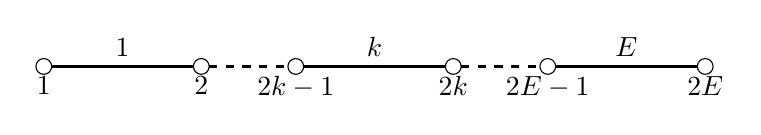
\begin{tikzpicture}
  \draw (2.3,0) circle (0.1) node [below] {$1$};
  \draw (4.3,0) circle (0.1) node [below] {$2$};
  \draw[thick] (2.4,0) -- (4.2,0) node [above,midway] {$1$};
  \draw[thick,dashed] (4.4,0) -- (5.4,0);
  \draw (5.5,0) circle (0.1) node [below] {$2k-1$};
  \draw (7.5,0) circle (0.1) node [below] {$2k$};
  \draw[thick] (5.6,0) -- (7.4,0) node [above,midway] {$k$};
  \draw[thick,dashed] (7.6,0) -- (8.6,0);
  \draw (8.7,0) circle (0.1) node [below] {$2E-1$};
  \draw (10.7,0) circle (0.1) node [below] {$2E$};
  \draw[thick] (8.8,0) -- (10.6,0) node [above,midway] {$E$};
\end{tikzpicture}

  \caption{One-dimensional mesh made of $E$ elements of constant length $\Delta X = \frac{l}{E}$.}\label{fig:1Dmesh}
\end{figure}

Since fields are carried by particles, we seek for the scheme equation that gives the solution $\bar{Q}$ at a material point for a given time step, with respect to the solutions of other particles at previous time step. In this section, lower and case symbols are respectively devoted to nodes and material points. Furthermore, since we consider here scalar quantities, the information on nodes and particles can be written as subscripts without ambiguity. Hence, at the time step $n$, the solution at material point $I$ reads $Q^{n}_I$ and it is the same for nodes. Then, the cell containing a given particle $J$ will be denoted by $c(J)$ so that the nodes interacting with this particle are $2c(J)-1$ and $2c(J)$. At last, the linear shape functions defined in element $c(J)$ are:
\begin{equation}
S_{2c(J)-1}(X)= \frac{X^{2c(J)} - X}{\Delta X} \qquad S_{2c(J)}(X)= \frac{X -X^{2c(J)-1}}{\Delta X} \qquad X \in \[X^{2c(J)-1},X^{2c(J)}\]
\end{equation}
and $S_{i,J}$ is the shape function of node $i$ evaluated at the position of the $I$th material point.

\subsubsection*{Scheme equation: Euler time discretization}
\label{subsec:scheme_Euler}
The method followed to write the scheme equation is to trace backward the numerical procedure described in section \ref{sec:DGMPM} in order to get an expression of the form \eqref{eq:general_scheme} for the material point $I$:
\begin{equation}
\bar{Q}^{n+1}_I = H\(\bar{Q}^{n}_K\) \qquad  K=1,..,N_p
\end{equation} 
Quantities at time $t^{n+1}$ are obtained by interpolating nodal solutions of the discrete equation \eqref{eq:DGMPM_discrete} in the cell containing the $I$th particle by the projection \eqref{eq:DGMPM_node2points}: 
\begin{equation}
\bar{Q}^{n+1}_I = S_{2c(I)-1,I}\bar{q}_{2c(I)-1}^{n+1} + S_{2c(I),I}\bar{q}_{2c(I)}^{n+1} \label{eq:updated_MP}
\end{equation}
With the interface fluxes in the case of the linear scalar advection equation $\Fc_N =  (aq^*) N $, in which $q^*$ is the stationary solution of Riemann's problem at the cell interface and $N=\pm 1$ the outward unit normal, the discrete form \eqref{eq:DGMPM_discrete} leads to the following expressions of updated nodal values:
\begin{equation}
  \label{eq:nodal_discrete_forms}
  \begin{aligned}
    & \bar{q}_{2c(I)-1}^{n+1}= \bar{q}_{2c(I)-1}^{n} + \frac{\Delta t}{M^L_{2c(I)-1}}\( K_{2c(I)-1,j} a\bar{q}_{j}^{n}- a\rho \bar{q}_{2c(I)-1}^*N_{2c(I)-1} \)\\
    &\bar{q}_{2c(I)}^{n+1}= \bar{q}_{2c(I)}^{n} + \frac{\Delta t}{M^L_{2c(I)}}\( K_{2c(I),j} a\bar{q}_{j}^{n}- a\rho \bar{q}_{2c(I)}^*N_{2c(I)} \)
  \end{aligned}
\end{equation}
Equations \eqref{eq:nodal_discrete_forms} can be simplified by first noting that in a one-dimensional grid, the outward unit vectors are $N_{2c(I)-1}=-1$ and $N_{2c(I)}=1$. Then, provided linear shape functions, the lumped mass and the pseudo-stiffness matrices are:
\begin{align}
  & M^L_i = \sum_{J=1}^{N_p} S_{iJ} m_J \\
  & K_{2c(I)-1,j} = \sum_{J=1}^{N_p} \drond{S_{2c(I)-1,J}}{X} m_J S_{jJ} = -\sum_{J=1}^{N_p} \frac{m_J S_{jJ}}{\Delta X} \\
  & K_{2c(I),j} = \sum_{J=1}^{N_p} \drond{S_{2c(I),J}}{X} m_J S_{jJ} = \sum_{J=1}^{N_p} \frac{m_J S_{jJ}}{\Delta X} 
\end{align}
where $m_J$ is the mass of $J$th material point. The discontinuous approximation basis moreover yields a bloc diagonal pseudo-stiffness matrix so that one can write:
\begin{equation}
  \label{eq:block_diag_K}
  K_{i,j} \bar{q}_{j}^{n}= K_{i,2c(i)-1} \bar{q}_{2c(i)-1}^{n}+K_{i,2c(i)} \bar{q}_{2c(i)}^{n}
\end{equation}
Furthermore, the mass density can be replaced by $\rho = N_p^{c( I)} m_I/\Delta X$ where $N_p^{c( I)}$ is the number of particles in the cell that contains the $I$th material point. Since waves travel from left to right ($a>0$), the stationary solution is equal to the value at the upwind node of an interface, that is:
\begin{align}
  & q_{2c(I)-1}^* = \rho \bar{q}^n_{2c(I)-2}=  N_p^{c( I)}\frac{ m_I}{\Delta X}\bar{q}^n_{2c(I)-2} \\
  & q_{2c(I)}^* = \rho \bar{q}^n_{2c(I)} =  N_p^{c( I)}\frac{ m_I}{\Delta X} \bar{q}^n_{2c(I)} 
\end{align}

Gathering all the previous consideration and seeing that the definition of the mass density used implies that every particles in a given cell carry the same mass, equations \eqref{eq:nodal_discrete_forms} read:
\begin{equation}
  \label{eq:nodal_euler}
  \begin{aligned}
    & \bar{q}_{2c(I)-1}^{n+1}= \bar{q}_{2c(I)-1}^{n} - \frac{a\Delta t}{\Delta X}\( \frac{f_{c(I)}^{n} - N_p^{c( I)} \bar{q}^n_{2c(I)-2}}{\sum_{J=1}^{N_p^{c(I)}}  S_{2c(I)-1,J}}\)\\
    &\bar{q}_{2c(I)}^{n+1}= \bar{q}_{2c(I)}^{n} + \frac{a\Delta t}{\Delta X}\( \frac{f_{c(I)}^{n}- N_p^{c( I)}  \bar{q}^n_{2c(I)}}{\sum_{J=1}^{N_p^{c(I)}}  S_{2c(I),J}} \)
  \end{aligned}
\end{equation}
where $f_{c}^{n}=\sum_{L=1}^{N_p^{c}} \[S_{2c-1,L}\bar{q}_{2c-1}^{n}+ S_{2c,L}\bar{q}_{2c}^{n}\]$, is related to the volume fluxes contributions. Note also that the Courant number $a\Delta t/\Delta X$ arises. Introduction of those equation in the updated material point solution \eqref{eq:updated_MP} leads after some simplifications to:
\begin{equation}
  \label{eq:euler_before_mapping}
  \begin{split}
    \bar{Q}^{n+1}_I = S_{2c(I)-1,I}q^n_{2c(I)-1}  &+ S_{2c(I),I}\(1-\frac{a\Delta t}{\Delta X}\frac{N_p^{c(I)}}{\sum_J S_{2c(I),J}}\)q^n_{2c(I)} +N_p^{c(I)}\frac{a\Delta t}{\Delta X} \frac{S_{2c(I)-1,I}}{\sum_J S_{2c(I)-1,J}}q^n_{2c(I)-2} \\
    & + \frac{a\Delta t}{\Delta X}\(\frac{S_{2c(I),I}}{\sum_J S_{2c(I),J}}-\frac{S_{2c(I)-1,I}}{\sum_J S_{2c(I)-1,J}}\)f_{c(I)}^{n}
  \end{split}
\end{equation}
In equation \eqref{eq:euler_before_mapping} the solutions at nodes result from the convection step \eqref{eq:DGMPM_points2nodes}:
\begin{equation}
\bar{q}^{n}_{i} = \frac{\sum_K S_{iK}m_K \bar{Q}^n_{K}}{\sum_P S_{iP}m_P} = \frac{\sum_K S_{iK} \bar{Q}^n_{K}}{\sum_P S_{iP}} \label{eq:stab_mapping}
\end{equation}
In particular, the volume fluxes contributions can be written:
\begin{equation}
  f_{c}^{n}=\sum_{L=1}^{N_p^{c}}\[S_{2c-1,L}\frac{\sum_K S_{2c-1,K}\bar{Q}^n_{K}}{\sum_P S_{2c-1,P}}+ S_{2c,L}\frac{\sum_K S_{2c,K} \bar{Q}^n_{K}}{\sum_P S_{2c(L),P}} \]=\sum^{N_p}_{K=1}\(S_{2c-1,K} +S_{2c,K} \)\bar{Q}^n_{K} \label{eq:volume_fluxes_mapped}
\end{equation}
Thus, introduction of mappings \eqref{eq:stab_mapping} and \eqref{eq:volume_fluxes_mapped} in equation \eqref{eq:euler_before_mapping} and permutation of sums over $K$ and $i$ lead after some simplifications to the scheme equation:
\begin{equation}
  \begin{split}
    \bar{Q}^{n+1}_I = \sum_{K=1}^{N_p} \bar{Q}^{n}_K & \left\lbrace \vphantom{\frac{S_{2c(I)-1,K}}{\sum_P S_{2c(I)-1,P}}}S_{2c(I)-1,I}\frac{S_{2c(I)-1,K}}{\sum_P S_{2c(I)-1,P}} + S_{2c(I),I}\frac{S_{2c(I),K}}{\sum_P S_{2c(I),P}} \right. \\
    & -\frac{a\Delta t}{\Delta X}N_p^{c(I)}\frac{S_{2c(I),I}}{\sum_J S_{2c(I),J}}\frac{S_{2c(I),K}}{\sum_P S_{2c(I),P}}\\
    & + \frac{a\Delta t}{\Delta X}N_p^{c(I)} \frac{S_{2c(I)-1,I}}{\sum_J S_{2c(I)-1,J}}\frac{S_{2c(I)-2,K}}{\sum_P S_{2c(I)-2,P}} \\
    &\left.+ \frac{a\Delta t}{\Delta X}\[\frac{S_{2c(I),I}}{\sum_J S_{2c(I),J}}-\frac{S_{2c(I)-1,I}}{\sum_J S_{2c(I)-1,J}}\]\(S_{2c(I)-1,K} +S_{2c(I),K}\) \right\rbrace \label{eq:scheme_euler1}
  \end{split}
\end{equation}
Note that the last term of formula \eqref{eq:scheme_euler1} is non-zero if particles $K$ and $I$ share the same cell, and in that case the parenthesis is one. Hence, the scheme equation can be rewritten as:
\begin{equation}
  \label{eq:Euler_scheme}
  \begin{split}
    \bar{Q}^{n+1}_I = \sum_{K=1}^{N_p} \bar{Q}^{n}_K  &\left\lbrace\sum_{i=1}^{2E}S_{iK}\frac{S_{iI}}{\sum_J S_{iJ}}  + N_p^{c(I)}\frac{a\Delta t}{\Delta X} \[\frac{S_{2c(I)-1,I}}{\sum_{J}  S_{2c(I)-1,J}}\frac{S_{2c(I)-2,K}}{\sum_{J}  S_{2c(I)-2,J}}-\frac{S_{2c(I),I}S_{2c(I),K}}{\(\sum_{J}  S_{2c(I),J}\)^2}\]\right.\\
    & + \left.   \frac{a\Delta t}{\Delta X} \[\frac{S_{2c(K),I}}{\sum_{J}  S_{2c(K),J}}-\frac{S_{2c(K)-1,I}}{\sum_J S_{2c(K)-1,J}}\] \vphantom{\sum_{i=1}^{2E}}\right\rbrace
  \end{split}
\end{equation}
The first (\textit{resp. second}) brackets in equation \eqref{eq:Euler_scheme} involve shape functions that are non zero if material point $K$ and $I$ lie in adjacent cells (\textit{resp. the same cell}). Hence, the numerical domain of dependence of the DGMPM for scalar linear advection with covers two cells regardless of the number of material points. Moreover, the particular case of one material point lying in every cell leads to the simplified form: 
\begin{equation}
  \begin{split}
    \label{eq:Godunov}
    \bar{Q}^{n+1}_I = \bar{Q}^{n}_I\(1-\frac{a\Delta t}{\Delta X}\) +\frac{a\Delta t}{\Delta X} \bar{Q}^{n}_{I-1} 
  \end{split}
\end{equation}
which corresponds to the Godunov scheme. This result is due to the convective phase from particles to nodes \eqref{eq:DGMPM_points2nodes} which in the case of a one particle-per-cell discretization leads to a piecewise constant reconstruction of fields on the grid. However, the previous identification no longer holds for other distributions of material points within the computational grid. 

\subsubsection*{Scheme equation: RK2 time discretization}
\label{subsec:scheme_RK2}
The solution of the discrete system on the grid for the second-order Runge-Kutta time integration consists in the two-stages procedure \eqref{eq:DGMPM_discrete_RK2} which, particularizes at node $i$ for the one-dimensional scalar linear advection equation as:
\begin{subequations}
  \begin{alignat}{1}
    \label{eq:RK2_stage1}& \bar{q}^{n+1/2}_{i}  =\bar{q}^{n}_{i} + \frac{1}{2}\frac{\Delta t}{M^L_{i}} a \( \sum_{j=1}^{2E} K_{i,j} \bar{q}^n_{j} - q^{*,n}_{i}N_i \) \quad \text{(no sum on $i$)} \\
    \label{eq:RK2_stage2}& \bar{q}^{n+1}_{i}  =\bar{q}^{n}_{i} + \frac{\Delta t}{M^L_{i}} a \( \sum_{j=1}^{2E} K_{i,j} \bar{q}^{n+1/2}_{j} - q^{*,n+1/2}_{i}N_i \) \quad \text{(no sum on $i$)}
  \end{alignat}
\end{subequations}
This procedure can be seen as a recursive use of the Euler scheme \eqref{eq:nodal_euler} with suitable time step sizes. Indeed, the first stage \eqref{eq:RK2_stage1} yields the intermadiate nodal fields in cell $c(I)$:
\begin{equation}
  \label{eq:discrete_RK2_step1}
  \begin{aligned}
    &\bar{q}_{2c(I)-1}^{n+1/2}= \bar{q}_{2c(I)-1}^{n} - \frac{a\Delta t}{2\Delta X}\( \frac{f_{c(I)}^{n} - N_p^{c( I)} \bar{q}^n_{2c(I)-2}}{\sum_{J=1}^{N_p^{c(I)}}  S_{2c(I)-1,J}}\)\\
    &\bar{q}_{2c(I)}^{n+1/2}= \bar{q}_{2c(I)}^{n} + \frac{a\Delta t}{2\Delta X}\( \frac{f_{c(I)}^{n}- N_p^{c( I)}  \bar{q}^n_{2c(I)}}{\sum_{J=1}^{N_p^{c(I)}}  S_{2c(I),J}} \)
  \end{aligned}
\end{equation}
In addition, the second stage \eqref{eq:RK2_stage2} leads to the expressions of nodal quantities at the end of the time step:
\begin{equation}
  \label{eq:discrete_RK2_step2}
  \begin{aligned}
    &\bar{q}_{2c(I)-1}^{n+1}= \bar{q}_{2c(I)-1}^{n} - \frac{a\Delta t}{\Delta X}\( \frac{\sum_{L=1}^{N_p^{c(I)}}\[S_{2c(I)-1,L}\bar{q}_{2c(I)-1}^{n+1/2}+ S_{2c(I),L}\bar{q}_{2c(I)}^{n+1/2}\] - N_p^{c( I)} \bar{q}^{n+1/2}_{2c(I)-2}}{\sum_{J=1}^{N_p^{c(I)}}  S_{2c(I)-1,J}}\)\\
    &\bar{q}_{2c(I)}^{n+1}= \bar{q}_{2c(I)}^{n} + \frac{a\Delta t}{\Delta X}\( \frac{\sum_{L=1}^{N_p^{c(I)}}\[S_{2c(I)-1,L}\bar{q}_{2c(I)-1}^{n+1/2}+ S_{2c(I),L}\bar{q}_{2c(I)}^{n+1/2}\]- N_p^{c( I)}  \bar{q}^{n+1/2}_{2c(I)}}{\sum_{J=1}^{N_p^{c(I)}}  S_{2c(I),J}} \)
  \end{aligned}
\end{equation}
Then, combination of the interpolation from nodes to particles \eqref{eq:updated_MP} and equations \eqref{eq:discrete_RK2_step2} leads, after some simplifications, to the solution at material point $I$ and time step $n+1$:
\begin{equation}
  \begin{split}
    \bar{Q}^{n+1}_I =  &S_{2c(I)-1,I}\bar{q}_{2c(I)-1}^{n} - \(\frac{a\Delta t}{\Delta X}\[S_{2c(I)-1,I} - S_{2c(I),I}\frac{\sum_{L} S_{2c(I)-1,L}}{\sum_{J}  S_{2c(I),J}}\] \)\bar{q}_{2c(I)-1}^{n+1/2} \\ & +S_{2c(I),I}\bar{q}_{2c(I)}^{n} + \frac{a\Delta t}{\Delta X}\[S_{2c(I),I} - S_{2c(I)-1,I}\frac{\sum_{L} S_{2c(I),L}}{\sum_{J}  S_{2c(I)-1,J}}- N_p^{c(I)}\frac{S_{2c(I),I}}{\sum_{J}  S_{2c(I),J}}\] \bar{q}_{2c(I)}^{n+1/2}\\
    &+N_p^{c(I)}\frac{a\Delta t}{\Delta X}\frac{S_{2c(I)-1,I}}{\sum_{J}  S_{2c(I)-1,J}}\bar{q}_{2c(I)-2}^{n+1/2}
  \end{split}
\end{equation}
Note that the volume fluxes contributions $f_c^{n}$ are used in equations \eqref{eq:discrete_RK2_step1} and not in \eqref{eq:discrete_RK2_step2}. Indeed, nodal values $q_i^{n+1/2}$ provided by the first stage of RK2 algorithm are substituted in the second one, it is therefore better to make them appear explicitly. It thus comes:
\begin{equation}
  \begin{split}
    \bar{Q}^{n+1}_I &=  S_{2c(I)-1,I}\bar{q}_{2c(I)-1}^{n} +S_{2c(I),I}\bar{q}_{2c(I)}^{n} \\
    &- \frac{a\Delta t}{\Delta X}\[S_{2c(I)-1,I} - S_{2c(I),I}\frac{\sum_{J} S_{2c(I)-1,J}}{\sum_{J}  S_{2c(I),J}}\] \(\bar{q}_{2c(I)-1}^{n} - \frac{a\Delta t}{2\Delta X}\( \frac{f_{c(I)}^{n} - N_p^{c( I)} \bar{q}^n_{2c(I)-2}}{\sum_{J}  S_{2c(I)-1,J}}\)\) \\
    &  + \frac{a\Delta t}{\Delta X}\[S_{2c(I),I}\(1- \frac{N_p^{c(I)}}{\sum_{J}  S_{2c(I),J}}\) - S_{2c(I)-1,I}\frac{\sum_{J} S_{2c(I),J}}{\sum_{J}  S_{2c(I)-1,J}}\] \(\bar{q}_{2c(I)}^{n} + \frac{a\Delta t}{2\Delta X}\( \frac{f_{c(I)}^{n}- N_p^{c( I)}  \bar{q}^n_{2c(I)}}{\sum_{J}  S_{2c(I),J}} \)\)\\
    &+N_p^{c(I)}\frac{a\Delta t}{\Delta X}\frac{S_{2c(I)-1,I}}{\sum_{J}  S_{2c(I)-1,J}}\(\bar{q}_{2c(I)-2}^{n} + \frac{a\Delta t}{2\Delta X}\( \frac{f_{c(I)-1}^{n}- N_p^{c( I)-1}  \bar{q}^n_{2c(I)-2}}{\sum_{J}  S_{2c(I)-2,J}} \)\) \label{eq:Mp_before_mapping}
  \end{split}
\end{equation}
Note that the second equation of the set \eqref{eq:discrete_RK2_step1} is used for $q^{n+1/2}_{2c(I)-2}$ since it is the downwstream node of the adjacent cell $c(I)-1$. Hence, the number of material points lying in that cell $N_p^{c(I)-1}$ arises from the expression of the mass density. At last, by rearranging formula \eqref{eq:Mp_before_mapping} as:
\begin{equation}
  \begin{split}
    \bar{Q}^{n+1}_I =  &\(S_{2c(I)-1,I} -\frac{a\Delta t}{\Delta X}\[S_{2c(I)-1,I} - S_{2c(I),I}\frac{\sum_{J} S_{2c(I)-1,J}}{\sum_{J}  S_{2c(I),J}}\]\)\bar{q}_{2c(I)-1}^{n} \\
    +&\(S_{2c(I),I} + \frac{a\Delta t}{\Delta X}\[S_{2c(I),I}\(1-\frac{N_p^{c(I)}}{\sum_{J}  S_{2c(I),J}}\) - S_{2c(I)-1,I}\frac{\sum_{J} S_{2c(I),J}}{\sum_{J}  S_{2c(I)-1,J}}\]\) \bar{q}_{2c(I)}^{n} \\
    +&\frac{1}{2}\(\frac{a\Delta t}{\Delta X}\)^2\(N_p^{c( I)}\[\frac{S_{2c(I)-1,I}}{\sum_J S_{2c(I)-1,J}} - \frac{S_{2c(I),I}}{\sum_{J}  S_{2c(I),J}}\] +S_{2c(I),I} \(\frac{N_p^{c(I)}}{\sum_{J}  S_{2c(I),J}}\)^2\)\bar{q}_{2c(I)}^{n}\\
    +&N_p^{c( I)}\frac{a\Delta t}{\Delta X}  \[ \frac{S_{2c(I)-1,I}}{\sum_{J}  S_{2c(I)-1,J}}\(1 -   \frac{a\Delta t}{2\Delta X}\(1+\frac{N_p^{c( I)-1} }{\sum_{J}  S_{2c(I)-2,J}} \)\)+\frac{a\Delta t}{2\Delta X} \frac{S_{2c(I),I}}{\sum_{J}  S_{2c(I),J}}\]\bar{q}^n_{2c(I)-2}\\
    -&\frac{1}{2}\(\frac{a\Delta t}{\Delta X}\)^2 N_p^{c(I)}\frac{S_{2c(I),I}}{\(\sum_{J}  S_{2c(I),J}\)^2} f_{c(I)}^{n} +\frac{1}{2}\(\frac{a\Delta t}{\Delta X}\)^2N_p^{c(I)}\frac{S_{2c(I)-1,I}}{\sum_{J}  S_{2c(I)-1,J}}\frac{ f_{c(I)-1}^{n}}{\sum_{J}  S_{2c(I)-2,J}}
  \end{split}
\end{equation}
the use of convective phase equations \eqref{eq:stab_mapping} and \eqref{eq:volume_fluxes_mapped} allows to write:
\begin{equation}
  \begin{split}
    \bar{Q}^{n+1}_I =  &\sum_{K} Q_K^n  \left\lbrace \frac{S_{2c(I)-1,K}}{\sum_J S_{2c(I)-1,J}}\(S_{2c(I)-1,I} -\frac{a\Delta t}{\Delta X}\[S_{2c(I)-1,I} - S_{2c(I),I}\frac{\sum_{L} S_{2c(I)-1,L}}{\sum_{J}  S_{2c(I),J}}\]\)  \right. \\
    &+\frac{S_{2c(I),K}}{\sum_J S_{2c(I),J}}\(S_{2c(I),I} + \frac{a\Delta t}{\Delta X}\[S_{2c(I),I}\(1-\frac{N_p^{c(I)}}{\sum_{J}  S_{2c(I),J}}\) - S_{2c(I)-1,I}\frac{\sum_{L} S_{2c(I),L}}{\sum_{J}  S_{2c(I)-1,J}}\]\)  \\
    &+\frac{S_{2c(I),K}}{\sum_J S_{2c(I),J}}\frac{1}{2}\(\frac{a\Delta t}{\Delta X}\)^2\(N_p^{c( I)}\[\frac{S_{2c(I)-1,I}}{\sum_J S_{2c(I)-1,J}} - \frac{S_{2c(I),I}}{\sum_{J}  S_{2c(I),J}}\] +S_{2c(I),I} \(\frac{N_p^{c(I)}}{\sum_{J}  S_{2c(I),J}}\)^2\)  \\
    &+\frac{N_p^{c( I)} S_{2c(I)-2,K}}{\sum_J S_{2c(I)-2,J}}\frac{a\Delta t}{\Delta X} \[ \frac{S_{2c(I)-1,I}}{\sum_{J}  S_{2c(I)-1,J}}\(1 -   \frac{a\Delta t}{2\Delta X}\(1+\frac{N_p^{c( I)-1} }{\sum_{J}  S_{2c(I)-2,J}} \)\)+\frac{a\Delta t}{2\Delta X} \frac{S_{2c(I),I}}{\sum_{J}  S_{2c(I),J}}\]\\
    &+\frac{1}{2}\(\frac{a\Delta t}{\Delta X}\)^2 N_p^{c(I)}\left.\( \frac{\[S_{2c(I)-2,K} +S_{2c(I)-3,K} \]}{\sum_{J}  S_{2c(I)-1,J}\sum_{J}  S_{2c(I)-2,J}} S_{2c(I)-1,I}-\frac{\[S_{2c(I)-1,K} +S_{2c(I),K} \]}{\(\sum_{J}  S_{2c(I),J}\)^2} S_{2c(I),I}\)  \right\rbrace
  \end{split}
\end{equation}
% \begin{equation}
%   \begin{split}
%     \bar{Q}^{n+1}_I =  &\sum_{K} Q_K^n  \left\lbrace \sum_i S_{iK}\frac{S_{iI}}{\sum_J S_{iJ}}
%       +\frac{a\Delta t}{\Delta X}\[\frac{S_{2c(I),K}}{\sum_J S_{2c(I),J}}S_{2c(I),I}\(1-\frac{N_p^{c(I)}}{\sum_{J}  S_{2c(I),J}}\) -\frac{S_{2c(I)-1,K}}{\sum_J S_{2c(I)-1,J}}S_{2c(I)-1,I}\] \right.\\
%     &+\frac{a\Delta t}{\Delta X}\[\frac{S_{2c(I)-1,K}S_{2c(I),I}}{\sum_{J}  S_{2c(I),J}} - \frac{S_{2c(I),K}S_{2c(I)-1,I}}{\sum_{J}  S_{2c(I)-1,J}} + N_p^{c( I)} \frac{S_{2c(I)-2,K}}{\sum_J S_{2c(I)-2,J}}\frac{S_{2c(I)-1,I}}{\sum_{J}  S_{2c(I)-1,J}}\] \\
%     &+\frac{1}{2}\(\frac{a\Delta t}{\Delta X}\)^2\frac{S_{2c(I),K}}{\sum_J S_{2c(I),J}}N_p^{c( I)}\[ \frac{S_{2c(I)-1,I}}{\sum_J S_{2c(I)-1,J}} - \frac{S_{2c(I),I}}{\sum_{J}  S_{2c(I),J}} +N_p^{c(I)}\frac{S_{2c(I),I} }{\(\sum_{J}  S_{2c(I),J}\)^2} \]\\
%     &+\frac{1}{2}\(\frac{a\Delta t}{\Delta X}\)^2 \frac{S_{2c(I)-2,K}}{\sum_J S_{2c(I)-2,J}}N_p^{c( I)}\[ \frac{S_{2c(I),I}}{\sum_{J}  S_{2c(I),J}} - \frac{S_{2c(I)-1,I}}{\sum_{J}  S_{2c(I)-1,J}}\(1+\frac{N_p^{c( I)-1} }{\sum_{J}  S_{2c(I)-2,J}} \)\] \\
%     &-\frac{1}{2}\(\frac{a\Delta t}{\Delta X}\)^2 N_p^{c(I)}\left.\(\frac{\[ S_{2c(K),I} \]}{\(\sum_{J}  S_{2c(I),J}\)^2} + \frac{S_{2c(K)+1,I}}{\sum_{J}  S_{2c(I)-1,J}\sum_{L}  S_{2c(I)-2,L}} \) \right\rbrace
%   \end{split}
% \end{equation}
Once the previous formula is simplified, the one-dimensional scheme equation of the DGMPM with the RK2 time discretization can be written as:
\begin{equation}
  \label{eq:RK2_scheme}
  \begin{split}
    \bar{Q}^{n+1}_I =  &\sum_{K} Q_K^n  \left\lbrace \sum_i S_{iK}\frac{S_{iI}}{\sum_J S_{iJ}}
      +\frac{a\Delta t}{\Delta X}\[\frac{S_{2c(K),I}}{\sum_{J}  S_{2c(K),J}} - \frac{S_{2c(K)-1,I}}{\sum_{J}  S_{2c(K)-1,J}}\] \right.\\
    &+\frac{a\Delta t}{\Delta X}N_p^{c( I)}\[\frac{S_{2c(I)-1,I}}{\sum_{J}  S_{2c(I)-1,J}}\frac{S_{2c(I)-2,K}}{\sum_J S_{2c(I)-2,J}}-\frac{S_{2c(I),I}S_{2c(I),K}}{\(\sum_J S_{2c(I),J}\)^2}\] \\
    &+\frac{1}{2}\(\frac{a\Delta t}{\Delta X}\)^2N_p^{c( I)} \(\frac{S_{2c(I),K}}{\sum_J S_{2c(I),J}}-\frac{S_{2c(I)-2,K}}{\sum_J S_{2c(I)-2,J}}\)\[\frac{S_{2c(I)-1,I}}{\sum_J S_{2c(I)-1,J}} - \frac{S_{2c(I),I}}{\sum_{J}  S_{2c(I),J}}\]\\
    %&+\frac{1}{2}\(N_p^{c( I)}\frac{a\Delta t}{\Delta X}\)^2\frac{S_{2c(I),K}}{\(\sum_{J}  S_{2c(I),J}\)^2}\frac{S_{2c(I),I} }{\sum_J S_{2c(I),J}} - \frac{1}{2}\(\frac{a\Delta t}{\Delta X}\)^2N_p^{c( I)}\frac{S_{2c(K),I}}{\(\sum_{J}  S_{2c(I),J}\)^2} \\
    &+\frac{1}{2}\(\frac{a\Delta t}{\Delta X}\)^2N_p^{c( I)}\frac{S_{2c(K),I}}{\(\sum_{J}  S_{2c(I),J}\)^2} \[N_p^{c( I)}\frac{S_{2c(I),K} }{\sum_J S_{2c(I),J}}-1\]\\
    &+ \frac{1}{2}\(\frac{a\Delta t}{\Delta X}\)^2\frac{S_{2c(K)+1,I}N_p^{c(I)}}{\sum_{J}  S_{2c(I)-1,J}\sum_{J}  S_{2c(I)-2,J}} \left.\[ 1 - N_p^{c( I)-1}\frac{S_{2c(I)-2,K} }{\sum_{J}  S_{2c(I)-2,J}}\] \right\rbrace
    \end{split}
\end{equation}
The first braces of the latter scheme equation correspond to that obtained for the Euler algorithm \eqref{eq:Euler_scheme} while the second order terms are provided by the two-stages time integration.

\subsubsection*{The von Neumann linear stability analysis}
The scheme equations obtained above are written for simplicity:
\begin{equation}
\bar{Q}^{n+1}_I = \sum_{K=1}^{N_p} \bar{Q}^n_{K} D_{IK} \label{eq:scheme_Dpi}
\end{equation}
Moreover, the computational domain is repeated periodically by mapping it to the domain $[-l,0]$ so that the solution at material point $J$ and time step $n$ is expanded into a discrete Fourier basis of $2E+1$ harmonics over the domain $X \in \[-l,l\]$:
\begin{equation}
\bar{Q}^{n}_J = \sum_{j=-E}^{E}A_j^n e^{I J k_j \Delta X}
\end{equation}
with $A^n_j$, the magnitude of the $j$th harmonic at time step $n$, $I = \sqrt{-1}$, and $k_j$ a wave number. Introduction of this expansion in equation \eqref{eq:scheme_Dpi} yields:
\begin{equation}
A_j^{n+1} e^{I I k_j \Delta X} = \sum_{K=1}^{N_p} A_j^n D_{IK}e^{I K k_j \Delta X}\quad \forall j=-E,...,E
\end{equation}
The amplification factor between two time steps at a given point is defined as:
\begin{equation}
\frac{A_j^{n+1}}{A_j^n} = \sum_{K=1}^{N_p} e^{I (K -I)k_j \Delta X} D_{IK} \quad \forall j=-E,...,E \label{eq:fourier_expansion}
\end{equation}
A necessary condition to ensure the stability of a numerical scheme is that the amplification factor must be lower than one in modulus: $\abs{A^{n+1}/A^n} < 1$. This upper bound allows to ensure that eventual errors do not increase during the computation. For expression \eqref{eq:fourier_expansion}, this leads to:
\begin{equation}
 \abs{\sum_{K=1}^{N_p} e^{I (K -I)k_j \Delta X} D_{IK}} \leq \sum_{K=1}^{N_p} \abs{e^{I (K -I)k_j \Delta X} D_{IK}} = \sum_{K=1}^{N_p} \abs{D_{IK}}
\end{equation}
where the triangle inequality, and the unit modulus of the complex number $e^{I (K -I)k_j \Delta X}$ have been used.
Hence, the DGMPM scheme is stable for a given discretization if the Courant number is set so that the following condition is satisfied for all material points:
\begin{equation}
  \label{eq:stability} \sum_{K=1}^{N_p} \abs{D_{IK}} \leq 1 \quad \forall \: I = 1,...,N_p
\end{equation}
Hence, the stability of the scheme is ensured by using the lowest CFL number resulting from the solution of \eqref{eq:stability} for every material points. According to scheme equations \eqref{eq:Euler_scheme} or \eqref{eq:RK2_scheme}, such a stability condition can be very hard to deal with analytically for general discretizations. However, the particular configuration for which one single particle (equation \eqref{eq:Godunov}) lies in each cell can be studied analytically. In this case, condition \eqref{eq:stability} reads:
\begin{equation}
\sum_{K=1}^{N_p} \abs{D_{IK}} = \abs{1 - a\frac{\Delta t}{\Delta X} } +  \abs{ a\frac{\Delta t}{\Delta X} } \leq 1 \label{1ppc_stab}
\end{equation}
which is satisfied for all $a\frac{\Delta t}{\Delta X} \leq 1$ regardless of the positions of particles. As it as been seen in section \ref{subsec:scheme_Euler}, the combination of DGMPM and first order Euler discretizations yields Godunov's scheme that is characterized by this stability condition. 
\begin{table}[h]
  \centering
  \input{chapter3/tabular/CFL_comparison_figures}
  \caption{DGMPM critical Courant numbers values for Euler or RK2 time integration with respect of the number and positions of material points in a one-dimensional grid. Black circles denote material points while white ones represent grid nodes.}
  \label{tab:CFL_comparison}
\end{table}
Although the infinity of possible material points distributions prevents the explicit derivation of a general stability condition, the optimal CFL number satisfying the equality in equation \eqref{eq:stability} can be find numerically. Some configurations are studied in table \ref{tab:CFL_comparison} and the critical Courant number resulting from the two time discretizations studied above are compared for each. Those results have been obtained by assuming that the particle distribution is the same in every element of a one-dimensional regular mesh so that a material point $I$ must lie between the nodes of the cell it belongs to, that is, $X^I \in \[X^{2c-1},X^{2c}\]$. First, the DGMPM scheme is stable for all CFL number lower to or equal one when cells contain one particle only regardless of their Positions. Then, when many material points share the same element, several configurations are considered:
\begin{itemize}
\item[(i)] particles are positioned symmetrically with respect to cells centers and regularly spaced in the mesh. This space discretization is referred to as the natural configuration in the following.
\item[(ii)] particles initially symmetrically positioned are shifted of $\delta=\Delta X/10$ with respect to cells centers and regularly spaced in the mesh.
\item[(iii)] the same than (ii) with $\delta$ so that the first material point overlaps the left node.
\item[(iv)] the same than (ii) with $\delta$ so that the last material point overlaps the right node.
\item[(v)] particles are placed symmetrically with respect to cells centers but not regularly spaced in the mesh.
\item[(vi)] the same than (v) with the first and last particles overlapping left and right nodes of cells respectively.
\end{itemize}
RK2 results bad when the upwind material point move to the right
One can see in table \ref{tab:CFL_comparison} that the RK2 time discretization provides better results in terms of CFL number for the distributions of particles considered. However, a uniform translation of material points in the mesh leads to a decrease in the Courant number for both time integrations. Furthermore the impact of such a translation is more significant in the stream direction (\textit{i.e. cases (ii) and (iv)}) in such a way that the decline in CFL number is bigger than for an inverse stream direction (\textit{i.e. cases (iii)}). In the latter situation, the Euler algorithm provides even better results than in the natural configuration. One the other hand, particles distributions that conserve the symmetry with respect to cells centers lead to the optimal stability condition when using the RK2 time integration while the Euler CFL depends on the spacing between material points. More specifically, Euler algorithm leads to a vanishing CFL for the case (vi), thus preventing any simulation. Therefore, the distribution of material points, and hence the resulting quadrature, has an influence on the stability of the scheme. As a consequence, the optimal Courant number can be reached even with the Euler discretization, while the classical DGFEM scheme developed in \cite{Chavent_Salzano} is restricted to condition $\Delta t / \Delta X = \Oc(\sqrt{\Delta X})$. This limitation has been addressed by introducing slope limiters in order to remove non-physical oscillations in the vicinity of sharp solutions while providing high-order accuracy in smooth regions \cite{Chavent_Cockburn}. However, the stability of the method was still bounded by $CFL\leq 1/2$ and the scheme was first-order accurate. The use of a second-order Runge kutta \cite{DGFEM_CFL} allowed to achieve second-order accuracy of the scheme, but the stability condition then reduced to $CFL\leq1/3$. More recently, space–time DGFEM formulations \cite{ST_DGFEM1,ST_DGFEM2} provided the ability to relax constraints of pure space DGFEM and obtain a critical CFL at 1.

%%%
The von Neumann linear stability analysis performed in this section provides an explicit (nonlinear) condition \eqref{eq:stability} that must be satisfied in order to ensure the stability of the DGMPM schemes based on both Euler and RK2 time discretizations. First, this relation allows to fully exploit the ability of the method to rebuild the grid mesh arbitrarily. Indeed, after such a procedure, the number and positions of material points in grid cells can change and one must be able to adapt properly the CFL number so that the scheme remains stable. An advantage on the original MPM is hence highlighted since no stability condition exists for the method. Second, it has been shown that some DGMPM discretizations provide an improvement of the restrictive CFL number that applies to the DGFEM scheme. In particular, the optimal condition allowing to capture discontinuities ($CFL=1$) can be reached for several space-time discretizations. This property turns out to be a strength for the DGMPM since it aims at follow waves accurately.

One can imagine to place material points so that an optimal stability condition is reached by minimizing some functional contrained with the description of material boundaries.

\subsection{Two-dimensional stability analysis}
Euler + CTU
\subsubsection*{Model equation - Space discretization}

We consider the scalar linear advection equation for an arbitrary quantity $q=\rho \bar{q}$ moving at constant speeds $a,b \in \Rbb^{+*}$ in $X$ and $Y$ directions respectively in a homogeneous one-dimensional medium:
\begin{equation}
  \label{eq:2D_model_equation}
  \drond{\bar{q}}{t} + a\drond{\bar{q}}{X} + b\drond{\bar{q}}{Y}= 0
\end{equation}
Note that the flux functions are in that case $\bar{f}^X = a\bar{q}$ and $\bar{f}^Y = b\bar{q}$. The physical domain is discretized with $N_p$ material points arbitrarily distributed in $E$ four-nodes bilinear elements with constant size $\Delta X \times \Delta Y$. In analogy with the one-dimensional case, DG approximation amounts to duplicate nodes and hence edges connected to them as depicted in figure \ref{fig:2Dmesh}. Again, there is no empty cell inside the physical so that no hole is generated, and periodic boundary conditions are considered to simplify the analysis. Thus, equation \eqref{eq:2D_model_equation} is discretized with the discontinuous Galerkin material point method using Euler time integration.
\begin{figure}[h!]
  \centering
  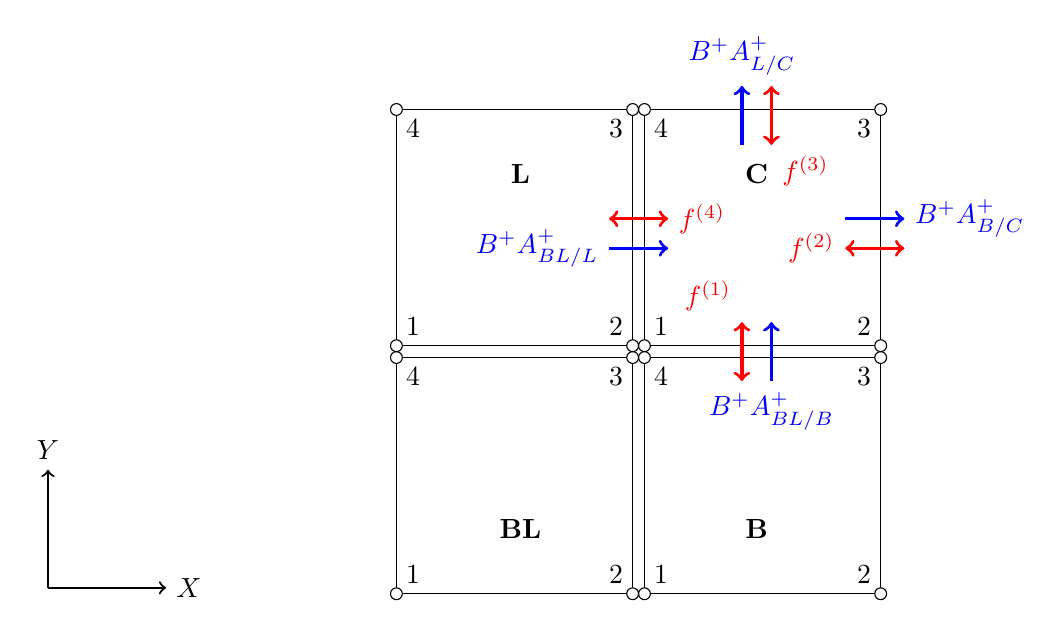
\begin{tikzpicture}[scale=1.5]
  \draw[thick,->] (-3,0.)-- (-2,0.) node[right] {$X$};
  \draw[thick,->] (-3,0.)-- (-3,1.) node[above] {$Y$};

  %% Cells
  \draw (0-0.05,0-0.05) rectangle (2.-0.05,2-0.05);
  \draw (0-0.05,2+0.05) rectangle (2.-0.05,4+0.05);
  \draw (2+0.05,0-0.05) rectangle (4.+0.05,2-0.05);
  \draw (2+0.05,2+0.05) rectangle (4.+0.05,4+0.05);
  %%%%%%%%%%%%%%%%%%%%%
  
  %% Nodes
  \fill[white] (0-0.05,0-0.05) circle (0.05);\fill[white] (2-0.05,2-0.05) circle (0.05);
  \fill[white] (0-0.05,2+0.05) circle (0.05);\fill[white] (2.-0.05,4+0.05) circle (0.05);
  \fill[white] (2+0.05,0-0.05) circle (0.05);\fill[white] (4.+0.05,2-0.05) circle (0.05);
  \fill[white] (2+0.05,2+0.05) circle (0.05);\fill[white] (4.+0.05,4+0.05) circle (0.05);
  \fill[white] (2-0.05,0-0.05) circle (0.05);\fill[white] (4.+0.05,0-0.05) circle (0.05);
  \fill[white] (0-0.05,2-0.05) circle (0.05);\fill[white] (2.+0.05,2-0.05) circle (0.05);
  \fill[white] (2-0.05,2+0.05) circle (0.05);\fill[white] (4.+0.05,2.+0.05) circle (0.05);
  \fill[white] (-0.05,4+0.05) circle (0.05);\fill[white] (2.+0.05,4+0.05) circle (0.05);

  \draw (0-0.05,0-0.05) circle (0.05) node[above right] {$1$};\draw (2-0.05,2-0.05) circle (0.05) node[below left] {$3$};
  \draw (0-0.05,2+0.05) circle (0.05) node[above right] {$1$};\draw (2.-0.05,4+0.05) circle (0.05) node[below left] {$3$};
  \draw (2+0.05,0-0.05) circle (0.05) node[above right] {$1$};\draw (4.+0.05,2-0.05) circle (0.05) node[below left] {$3$};
  \draw (2+0.05,2+0.05) circle (0.05) node[above right] {$1$};\draw (4.+0.05,4+0.05) circle (0.05) node[below left] {$3$};
  \draw (2-0.05,0-0.05) circle (0.05) node[above left] {$2$};\draw (4.+0.05,0-0.05) circle (0.05) node[above left] {$2$};
  \draw (0-0.05,2-0.05) circle (0.05) node[below right] {$4$};\draw (2.+0.05,2-0.05) circle (0.05) node[below right] {$4$};
  \draw (2-0.05,2+0.05) circle (0.05) node[above left] {$2$};\draw (4.+0.05,2.+0.05) circle (0.05) node[above left] {$2$};
  \draw (-0.05,4+0.05) circle (0.05) node[below right] {$4$};\draw (2.+0.05,4+0.05) circle (0.05) node[below right] {$4$};
  %%%%%%%%%%%%%%%%%%%%%%%

  %% Cells names
  \node at (3,3.5) {$\textbf{C}$};
  \node at (1,0.5) {$\textbf{BL}$};
  \node at (3,0.5) {$\textbf{B}$};
  \node at (1,3.5) {$\textbf{L}$};

  %% Transverse corrections
  \draw[->, very thick,Blue] (2.875,3.75) -- (2.875,4.25) node [above] {$B^+A^+_{L/C}$}; % Top
  \draw[->, very thick,Blue] (3.75,3.125) -- (4.25,3.125) node [right] {$B^+A^+_{B/C}$}; % Right
  \draw[<-, very thick,Blue] (3.125,2.25) -- (3.125,1.75) node [below] {$B^+A^+_{BL/B}$}; % Bottom
  \draw[<-, very thick,Blue] (2.25,2.875) -- (1.75,2.875) node [left] {$B^+A^+_{BL/L}$}; % Left

  %% Normal fluxes
  \draw[<->, very thick,Red] (3.125,3.75) node [below right] {$f^{(3)}$} -- (3.125,4.25) ; % Top
  \draw[<->, very thick,Red] (3.75,2.875) node [left] {$f^{(2)}$}-- (4.25,2.875) ; % Right
  \draw[<->, very thick,Red] (2.875,2.25) node [above left] {$f^{(1)}$}-- (2.875,1.75); % Bottom
  \draw[<->, very thick,Red] (2.25,3.125) node [right] {$f^{(4)}$} -- (1.75,3.125); % Left

  % %% Edges numbers
  % \node[above] at (1,-0.1) {$(1)$};
  % \node[left] at (2,1.) {$(2)$};
  % \node[below] at (1,1.95) {$(3)$};
  % \node[right] at (-0.1,1.) {$(4)$};
\end{tikzpicture}


%%% Local Variables:
%%% mode: latex
%%% TeX-master: "../../mainManuscript"
%%% End:

  \caption{Two-dimensional mesh made of $E$ elements of constant size $\Delta X \times \Delta Y$.}\label{fig:2Dmesh}
\end{figure}

\subsubsection*{Two-dimensional scheme equation}
\begin{equation}
  \bar{q}_i^{n+1} = \bar{q}_i^n + \frac{\Delta t}{M^L_i} \(K_{ij}^X a\bar{q}_j^n + K_{ij}^Y b\bar{q}_j^n - \hat{f}_i^{*}\) \label{eq:discrete2D}
\end{equation}
The interface flux at a given node $\hat{f}_i^{*}$ results from integration of Godunov's flux along the edge it belongs to, according to the weak form \eqref{eq:DGMPM_semi_discrete}. Considering egde $(i)$, equation \eqref{eq:2D_model_equation} yields the following Godunov's fluxes:
\begin{equation}
  \label{eq:2d_Godunov_fluxes}
  f^{*,(i)}= c_n q^{(i)}_L = \underbrace{c_nq^{(i)}_R}_{f_N(q^{(i)}_R)} - \underbrace{c_n (q^{(i)}_R -q^{(i)}_L)}_{A^{+}_{L/R}} 
\end{equation}
where $c_n$ is the speed in the direction normal to the edge (\textit{i.e. b for horizontal and a for vertical edges}), $q^{(i)}_L$ and $q^{(i)}_R$ denote state vectors obtained by averaging nodal values on upwind and downwind sides respectively, and $A_{L/R}^+$ is the right-going fluctuation at the edge shared by Left and Right cells. Transverse corrections are considered through fluctuations $B^+A^+_{i/j}$ according to equation \eqref{eq:transverse_fluctuations}:
\begin{equation}
  \label{eq:2D_transverse_corrections}
  B^+A^+_{i/j}=c_t c_n (q^{(i)}_R -q^{(i)}_L)
\end{equation}
with $c_t$ the speed in the direction tangent to the edge.
Consider the edge $(1)$ of cell $C$:
\begin{equation}
  f^{*,(1)} = b \frac{q_3^{B,n} + q_4^{B,n}}{2} + a b \frac{\Delta t}{2\Delta Y}\(\frac{q_1^{B,n}+q_4^{B,n}}{2}-\frac{q_2^{BL,n}+q_3^{BL,n}}{2}\)
\end{equation}
where the first term corresponds to the flux of the upwind state and the second one in the transverse contribution of the right-going fluctuation at the edge between by Bottom ($B$) and Bottom-Left ($BL$) cells. Similarly, the other interface fluxes of that cell are:
\begin{align}
  & f^{*,(2)} = a \frac{q_2^{C,n} + q_3^{C,n}}{2} - a b \frac{\Delta t}{2\Delta X}\(\frac{q_1^{C,n}+q_2^{C,n}}{2}-\frac{q_3^{B,n}+q_4^{B,n}}{2}\) \\
  & f^{*,(3)} = b \frac{q_3^{C,n} + q_4^{C,n}}{2} - a b \frac{\Delta t}{2\Delta Y}\(\frac{q_1^{C,n}+q_4^{C,n}}{2}-\frac{q_2^{L,n}+q_3^{L,n}}{2}\) \\
  & f^{*,(4)} = a \frac{q_3^{C,n} + q_4^{C,n}}{2} + a b \frac{\Delta t}{2\Delta X}\(\frac{q_1^{L,n}+q_2^{L,n}}{2}-\frac{q_3^{BL,n}+q_4^{BL,n}}{2}\)
\end{align}
Introduction of the convective phase where $Q_I=\rho \bar{Q}_I= \frac{m_I N_p}{\Delta X \Delta Y}\bar{Q}_I$ with no sum on $I$:
\begin{align}
  & f^{*,(1)} = \sum_{J=1}^{N_p}\bar{Q}_J^n\frac{b N_p m_J }{2\Delta X \Delta Y} \left\lbrace  \(\frac{S_{3J}^{B} }{\sum_P S_{3P}^{B}} + \frac{S_{4J}^{B}}{\sum_PS_{4P}^{B}}\) + a  \frac{\Delta t}{2\Delta Y}\(\frac{S_{1J}^{B}}{\sum_P S_{1P}^B} + \frac{S_{4J}^{B}}{\sum_PS_{4P}^{B} }-\frac{S_{2J}^{BL}}{\sum_P S_{2P}^{BL}} + \frac{S_{3J}^{BL}}{\sum_PS_{3P}^{BL}}\) \right\rbrace\\
  & f^{*,(2)} = \sum_{J=1}^{N_p} \bar{Q}_J^n\frac{a N_pm_J }{2\Delta X \Delta Y} \left\lbrace  \(\frac{S_{2J}^{C}}{\sum_P S_{2P}^{C}} + \frac{S_{3J}^{C}}{\sum_P S_{3P}^{C}} \)- b \frac{\Delta t}{2\Delta X}\(\frac{S_{1J}^{C}}{\sum_P S_{1P}^{C}} + \frac{S_{2J}^{C}}{\sum_P S_{2P}^{C}}-\frac{S_{3J}^{B}}{\sum_P S_{3P}^{B}} +\frac{S_{4J}^{B}}{\sum_P S_{4P}^{B}}\) \right\rbrace\\
  & f^{*,(3)} =\sum_{J=1}^{N_p}\bar{Q}_J^n\frac{b N_pm_J }{2\Delta X \Delta Y} \left\lbrace  \(\frac{S_{3J}^{C}}{\sum_P S_{3P}^{C}} + \frac{ S_{4J}^{C}}{\sum_P S_{4P}^{C}}\) - a  \frac{\Delta t}{2\Delta Y}\(\frac{S_{1J}^{C}}{\sum_P S_{1P}^{C}} + \frac{S_{4J}^{C}}{\sum_P S_{4P}^{C}}-\frac{S_{2J}^{L}}{\sum_P S_{2P}^{L}} + \frac{S_{3J}^{L}}{\sum_P S_{3P}^{L}}\) \right\rbrace\\
  & f^{*,(4)} = \sum_{J=1}^{N_p}\bar{Q}_J^n\frac{a N_pm_J }{2\Delta X \Delta Y}  \left\lbrace  \(\frac{S_{3J}^{C}}{\sum_P S_{3P}^{C}} + \frac{ S_{4J}^{C}}{\sum_P S_{4P}^{C}}\) + b \frac{\Delta t}{2\Delta X}\(\frac{S_{1J}^{L}}{\sum_P S_{1P}^{L}} + \frac{S_{2J}^{L}}{\sum_P S_{2P}^{L}}-\frac{S_{3J}^{BL}}{\sum_P S_{3P}^{BL}} + \frac{S_{4J}^{BL}}{\sum_P S_{4P}^{L}}\)\right\rbrace
\end{align}
which will be written for simplicity: $f^{*,(i)}=\sum_J \bar{Q}_J^n \frac{c_n N_p m_J}{2\Delta X \Delta Y}\( \phi_J^{(i)} +\phi_J^{(i),T} \)$ where $\phi^{(i)}$ and $\phi^{(i),T}$ stand for normal and transverse fluxes contribution at edge $(i)$.

Thus, considering the cartesian grid shown in figure \ref{fig:2Dmesh}, the interface flux contribution at node $i$ is:
\begin{equation}
  \label{eq:nodal_fluxes}
  \hat{f}_i^{*} = \sum_j \int_{(j)}S_i(X,Y) f^{*,(j)}  \(N^{(j)}_X+N^{(j)}_Y\) dY =
  \left\lbrace
  \begin{aligned}
    & N^{(j)}_X \frac{l^{(j)}}{2} f^{*,(j)} \quad \text{if (j) is vertical}\\
    & N^{(j)}_Y \frac{l^{(j)}}{2} f^{*,(j)} \quad \text{if (j) is horizontal}
  \end{aligned}
  \right.
\end{equation}
where $N^{(j)}_X$ and $N^{(j)}_Y$ are the components of the outwerd normal vector to edge $(j). $Note that in the Cartesian grid, $N^{(j)}_X+N^{(j)}_Y = \pm 1$ gives the sign of the contribution of the interface flux to the node. In order to write a generic form of the nodal fluxes \eqref{eq:nodal_fluxes} that uses sums over every edge of the domain, the use of the shape function attached to node $i$ evaluated at edge centroids $S_{i}(\vect{X}^{(j)}_c)$ is made. Then, denoting the length of edge $(j)$ by $l^{(j)}$, it comes:
\begin{equation}
  \label{eq:nodal_flux_sum}
  \hat{f}^*_i = \sum_{j=1}^{\text{edges}} S_{i}(\vect{X}^{(j)}_c) l^{(j)}\(N_X^{(j)}+N^{(j)}_Y\) f^{*,(j)}
\end{equation}
\begin{equation}
  \label{eq:nodal_fluxe_mapped}
  \hat{f}_i^{*}=\sum_P \bar{Q}_P^n  \sum_{j=1}^{\text{edges}} S_{i}(\vect{X}^{(j)}_c) l^{(j)}\(a N_X^{(j)}+ bN^{(j)}_Y\)\frac{N^C_p m_J}{2\Delta X \Delta Y}\[\phi_P^{(j)} + \phi_P^{(j),T}\] 
\end{equation}
In the discrete form, those terms are divided by the lumped mass matrix:
\begin{equation}
  \hat{f}_i^{*}=\sum_P \frac{\bar{Q}_P^n}{\sum_J S_{iJ}}   \sum_{j=1}^{\text{edges}} S_{i}(\vect{X}^{(j)}_c) l^{(j)}\(aN_X^{(j)}+bN^{(j)}_Y\)\frac{N_p^C }{2\Delta X \Delta Y}\[\phi_P^{(j)} + \phi_P^{(j),T}\] 
\end{equation}
Si la grille n'est pas régulière, on ne garde qu'un $1/\Delta X$ et les contributions transverses approtent une correction d'ordre 2 en temps.

Making use of parent coordinates $(\xi,\eta)$, defined in cell $C$ as:
\begin{align}
  &\xi = 2\frac{X-X^C_1}{\Delta X} -1 \quad ; \quad d\xi = 2\frac{dX}{\Delta X} \label{ref_elemx}\\
  &\eta = 2\frac{Y-Y^C_1}{\Delta X} -1 \quad ; \quad d\eta = 2\frac{dY}{\Delta Y} \label{ref_elemy}
\end{align}
and the chain rule, the pseudo-stiffness matrices read:
\begin{align}
  & K_{ij}^X = \sum_J \drond{S_{iJ}}{X}m_JS_{jJ}=\frac{2}{\Delta X}\sum_J\drond{S_{iJ}}{\xi}m_JS_{jJ} =\frac{2}{\Delta X}\sum_J\nabla_\xi S_{iJ} m_J S_{jJ}\\
  &K_{ij}^Y = \sum_J\drond{S_{iJ}}{Y}m_JS_{jJ}=\frac{2}{\Delta Y}\sum_J\drond{S_{iJ}}{\eta}m_JS_{jJ} =\frac{2}{\Delta Y}\sum_J\nabla_\eta S_{iJ}m_J S_{jJ}
\end{align}
Then, the discrete equation \eqref{eq:discrete2D} can be rewritten by introducing:
\begin{align}
  & \frac{K_{ij}^X}{M_i^L}  =  \frac{2}{\Delta X} \frac{\sum_J\nabla_\xi S_{iJ}  S_{jJ}}{\sum_P  S_{iP}}=\frac{2}{\Delta X} k^X_{ij} \\
  & \frac{K_{ij}^Y}{M_i^L} = \frac{2}{\Delta X} \frac{\sum_J\nabla_\eta S_{iJ} S_{jJ}}{\sum_P S_{iP}} = \frac{2}{\Delta Y}  k^Y_{ij}
\end{align}
The solution at material points contained in cell $C$ at time step $n+1$ result from the interpolation of updated nodal quantities:
\begin{equation}
  \label{eq:2Dupdated_MP}
  \bar{Q}_I^{n+1}= S_{iI}\bar{q}_i^n + \Delta t S_{iI} \(  2\frac{a\Delta}{\Delta X} k^X_{ij}\bar{q}_j^n +  2\frac{b\Delta t}{\Delta Y} k^Y_{ij}\bar{q}_j^n - \frac{\hat{f}_i^{*}}{M_i^L}\)
\end{equation}
where:
\begin{equation}
  \frac{\hat{f}_i^{*}}{M_i^L}=\sum_J \frac{\bar{Q}_J^n}{\sum_P S_{iP}}  \frac{N_p}{4}\left\lbrace b\frac{\Delta t}{\Delta Y} N^3_Y\( \phi^{(3)} + \phi^{(3),T} \) + a\frac{\Delta t}{\Delta X} N^4_X\( \phi^{(4)} + \phi^{(4),T} \) \right\rbrace
\end{equation}

\subsubsection*{The von Neumann linear stability analysis}

\subsection{Non-linear stability analysis}
Convergence to entropy solution ; Non-linear stability ; entropy inequality
see \cite[p.219]{Leveque}, where lax entropy condition may be used instead of such an entropy inequality

Convergence in linear case is just mentioned and not shown in \cite{Cockburn}. But for non-linear cases it is based on the entropy inequality.

%% Test diffusion with limiters influence in the test case riemann_prob.py in DGMPM/elasticity
\subsection{Convergence analysis}
see Roe theorem \cite[p.417]{Toro}


Pfffff, franchement on peut en parler mais c'est bien relou à interpréter tellement ça dépend de la discretisation. On peut par exemple montrer qu'on est monotone pour 1ppc (FOU method) donc ordre 1. On peut aussi dire que ce n'est pas évident pour 2ppc. Après avoir dit ça, tracer des courbes de convergences paraît futile. Donc ça implique de développer la scheme equation, faire la stabiliter pour bien buter tout le monde et finir par la convergence.

%%% Local Variables: 
%%% mode: latex
%%% TeX-master: "../mainManuscript"
%%% End:
